\section{Hubs and high fares: Borenstein (1989)}\label{sec:09-borenstein}

\citet{Borenstein1989} asks whether the dominance of a route or of an airport lets a carrier raise its fares,
and whether its rivals benefit when it does. The paper is a reduced-form study. It regresses fares on measures
of market structure, cost and service quality across a large cross-section of routes. It reads the
coefficients through pricing theory of the kind developed in \cref{sec:09-pricing}. We follow the paper from
its question to its contribution, derive its estimating equations and instruments, and reproduce its four
tables. \Cref{tab:09-bor-map} at the end of the section maps the study. As in the rest of the chapter, $f$ indexes carriers and $t$ indexes routes, which here are directional
airport pairs.\footnote{Borenstein indexes airlines by $i$ and routes by $j$. He writes the coefficients of his
equation (1) as $\alpha_i$, $\beta_1$, $\gamma_1,\dots,\gamma_6$, $\delta_1,\dots,\delta_6$ and
$\rho_1,\dots,\rho_{24}$. We write $a_f$, $b_D$, $\gamma_1,\dots,\gamma_6$, $\phi_1,\dots,\phi_6$ and
$\varrho_1,\dots,\varrho_{24}$, because $\alpha$, $\beta$, $\delta$ and $\rho$ have other meanings in this
book. Page numbers in this section refer to the journal pages of the article.}

\subsection{The question}\label{sec:09-bor-question}

By the late 1980s it was well established that airline fares do not behave as the contestability benchmark
predicts. Fares on a route rise with the route's concentration
\citep{GrahamKaplanSibley1983,BaileyGrahamKaplan1985,CallKeeler1985,MorrisonWinston1987}. This finding
contradicts prediction (C1) of \cref{sec:09-contest-fail}, but it leaves open the source of the market power.
The traditional reading is that concentration makes tacit or explicit collusion easier. Borenstein proposes a
second source, the size of a carrier's operations at the endpoints of a route \citep[pp.~344--345]{Borenstein1989}.

The question has two parts. The first concerns a carrier's own fares. Holding costs and service quality fixed,
does a carrier charge more when it carries a larger share of a route's passengers? Does it charge more when it
carries a larger share of the passengers who begin their trips at the route's endpoint airports? The second part concerns its rivals. Do the
high fares of a dominant carrier create an \emph{umbrella effect}, a shelter under which the smaller carriers
on the same route can also price high? Collusion theories predict an umbrella, since every firm in a
concentrated market shares in the collusive price. Theories in which dominance is an advantage specific to one
carrier predict none.

The answer matters for policy. If concentration facilitates collusion, the relevant market structure is the
route, and policy should keep routes unconcentrated. If dominance of an airport is the source, the relevant
structure is the hub. A merger that raises a carrier's share of an airport can then raise fares on every route
from that airport. The mergers of 1986 and 1987 raised exactly this issue (\cref{sec:09-hubs}), and Borenstein
draws much of his anecdotal evidence from their regulatory dockets.

The answer, stated in the abstract (p.~344), has two parts. A carrier's share of the passengers on a route and
its share of the passengers at the endpoint airports both raise its markup over cost significantly. The high
markups of a dominant carrier, however, create little umbrella for carriers with smaller operations in the same
markets. The paper offers several explanations for this asymmetry, all of which work through advantages
specific to the dominant carrier.

\subsection{Setting}\label{sec:09-bor-setting}

\Cref{sec:09-dominance-sources} described the mechanisms through which airport dominance may confer market
power. They are reputation, frequent-flyer programs, travel agent commission overrides, biased reservation
systems, and control of gates and slots. All of them favor the carrier with the most flights at an airport, and
all of them act on every route that touches the airport. They therefore predict an effect of a carrier's
airport share on its fares that is distinct from the effect of its route share. They also predict that the
airport effect is strongest for the fares paid by business travelers, who belong to frequent-flyer programs and
are least sensitive to price.

Testimony in the merger cases illustrates the mechanisms. In the USAir-Piedmont case, Piedmont's
vice-president for planning stated that Piedmont would never consider entering the route from Pittsburgh to
Washington National (p.~345, n.~2). The reason was USAir's dominant position at Pittsburgh. He added that Piedmont
might compete with USAir from its own hub at Baltimore to Pittsburgh, because ``that is strength against
strength.'' The testimony suggests that presence at the endpoints of a route governs who serves it. Borenstein
exploits this link to construct his instrument for route share (\cref{sec:09-bor-ident}).

Two further features of the setting shape the design. First, airport capacity was scarce at several large
airports. Part of a high fare at such an airport may be a competitive scarcity rent common to all carriers
there. The design must separate it from carrier-specific market power (\cref{eq:09-scarcity}). Second,
several cities have more than one airport. Borenstein treats flights from different airports as separate
markets and leaves their substitutability for future work (p.~348).

\Cref{sec:09-pricing} provides two models that frame the empirical work. In the conduct model behind
\cref{eq:09-pricing-approx}, a carrier's log price rises linearly in its route share, and a degree of
collusiveness that rises with concentration produces an umbrella. In the logit model of
\cref{prop:09-dominance}, an increase in one carrier's attractiveness raises its own price and share and lowers
the prices of its rivals. Borenstein's two estimating equations are built to discriminate between these
predictions.

\subsection{Data}\label{sec:09-bor-data}

\casehead{Sources and sample} The data cover the third quarter of 1987. Fares and passenger counts come from
the DB1A ticket sample, flight operations from the Service Segment Data, and enplanements from the Nonstop
Market Data (\cref{sec:09-data}). Costs per available seat-mile come from the DOT's \emph{Air Carrier Traffic
Statistics} and \emph{Air Carrier Financial Statistics}. Populations come from the \emph{Statistical Abstract of
the United States} and the tourism index from the \emph{Census of Service Industries} (pp.~363--364). The ticket
conventions are those of \cref{sec:09-data}. Round trips count as two directional trips at half fare each, and
first-class, interline, international and sub-\$10 tickets are dropped. Tickets that use a segment missing from
the Service Segment Data, fewer than 1\% of passengers, are also dropped (p.~362).

The sample covers the nine largest domestic carriers, namely American, USAir, Continental, Delta, Eastern,
Northwest, Piedmont, TWA and United (p.~349, n.~20). Continental and Eastern belonged to one holding company,
Texas Air. They operated as separate companies with different costs, reputations and regions, and Borenstein
treats them as separate firms. Only local passengers count toward a route. A local passenger's ticket begins
at one endpoint and ends at the other, with at most one change of plane in each direction (p.~349, n.~21).
Through and connecting passengers, for whom an endpoint is neither origin nor destination, do not count.

The nine carriers served 5,428 routes. On 3,591 of them, at least one of the nine carriers held at least 10\%
of the route's passengers and carried at least 10 passengers per day. These routes form the sample for the
pricing equation. On 1,508 routes at least two carriers met both criteria, and these routes form the sample
for the relative-price equation (p.~355). The unit of observation is a carrier-route pair. When several
carriers qualify on a route, Borenstein keeps one of them, drawn at random, because the errors of different
carriers on the same route are unlikely to be independent (p.~354). The pricing sample therefore has one
observation per route.

\casehead{Dependent variables} For each carrier-route pair, sort the fares paid by the carrier's passengers
from lowest to highest, counting each fare once per passenger. FR20, FR50 and FR80 are the 20th, 50th and 80th
percentiles of this passenger-weighted distribution (p.~348, n.~19). The three percentiles serve two purposes.
The median is less sensitive than the mean to reporting errors. The three points also let every coefficient
differ between deeply discounted fares and the high fares that business travelers tend to pay. Each regression
uses the log of one percentile as its dependent variable.

\Cref{tab:09-bor-desc} reports summary statistics for the pricing sample. The mean 80th-percentile fare, \$187,
is 1.86 times the mean 20th-percentile fare, which shows how much fares vary within a carrier-route pair. The
observed carrier's mean route share is 0.54. It is high because a carrier enters the sample only if it holds at
least 10\% of the route. The mean airport origination share is 0.24 and the mean route Herfindahl index is
0.50. A typical observation involves 0.67 changes of plane per passenger and routings 7.5\% longer than the
nonstop distance. Delta supplies the most observations (18\%) and TWA the fewest (5\%).

\begin{table}[htbp]
\centering
\caption{Summary statistics of the pricing-equation sample}
\label{tab:09-bor-desc}
\footnotesize
\begin{tabular}{@{}llrrrr@{}}
\toprule
Variable & Unit & Mean & Std.\ dev. & Minimum & Maximum \\
\midrule
FR20 & dollars & 100.39 & 35.03 & 22.00 & 329.00 \\
FR50 & dollars & 129.44 & 42.80 & 27.00 & 359.00 \\
FR80 & dollars & 187.20 & 64.51 & 38.00 & 537.00 \\
DISTANCE & miles & 1,084.31 & 735.56 & 104.00 & 5,083.00 \\
LOADFAC & fraction of seats & 0.6055 & 0.0973 & 0.1225 & 0.9098 \\
EQUIP & seats per plane & 112.75 & 27.89 & 60.00 & 271.90 \\
FREQ & flights per quarter & 625.91 & 296.73 & 10.00 & 2,892.00 \\
CIRC & ratio & 1.0754 & 0.1169 & 1.0000 & 1.9004 \\
STOP & stops per passenger & 0.0765 & 0.1403 & 0.0000 & 1.3700 \\
PLANECHG & changes per passenger & 0.6708 & 0.4174 & 0.0000 & 1.0000 \\
ORGSHARE & fraction & 0.2422 & 0.1305 & 0.0212 & 0.8647 \\
ORGHERF & index & 0.2541 & 0.0961 & 0.1158 & 0.8622 \\
RUTSHARE & fraction & 0.5419 & 0.2656 & 0.1003 & 1.0000 \\
RUTHERF & index & 0.4954 & 0.2237 & 0.1266 & 1.0000 \\
COMPCOST & dollars per seat-mile & 0.0813 & 0.0061 & 0.0476 & 0.1037 \\
TOURIST & ratio & 0.0141 & 0.0144 & 0.0028 & 0.0700 \\
POTCOMP & fraction & 0.1590 & 0.1592 & 0.0000 & 0.8259 \\
GENPSH & fraction & 0.3752 & 0.2344 & 0.0238 & 1.0000 \\
TOTMILE & miles & 1,145.45 & 750.94 & 105.00 & 5,176.00 \\
\bottomrule
\end{tabular}

\smallskip
\begin{minipage}{0.92\linewidth}
\footnotesize Notes: 3,591 carrier-route observations, third quarter of 1987. Values are rounded from the
paper, which prints more digits. The paper labels the instrument GENPSH as GEOENPSH in this table. TOTMILE is
the average total routing mileage, so $\mathit{CIRC} = \frac{\mathit{TOTMILE}}{\mathit{DISTANCE}}$. Shares of
observations by carrier: American 0.140, USAir 0.101, Continental 0.141, Delta 0.180, Eastern 0.072, Northwest
0.094, Piedmont 0.110, TWA 0.051, United 0.111. The table also reports the means of the 24 airport scarcity
variables, which are omitted here. Source: \citet{Borenstein1989}, Table 4.
\end{minipage}
\end{table}

\casehead{Descriptive evidence} Before any regression, \citet[Table 1]{Borenstein1989} compares yields, that
is, fares per mile, at six airports dominated by one carrier. \Cref{tab:09-bor-yields} reproduces the table and
\cref{fig:09-bor-yields} plots it. For each airport the table gives three yields. The first is the dominant
carrier's yield on routes to or from the airport. The second is the same carrier's yield on the rest of its
system, and the third is the yield of other carriers on routes to or from the airport. Yields are reported by
band of nonstop distance and over all distances.

\begin{table}[htbp]
\centering
\caption{Yields at six dominated airports, third quarter of 1987 (cents per mile)}
\label{tab:09-bor-yields}
\footnotesize
\setlength{\tabcolsep}{4.2pt}
\begin{tabular}{@{}lrrrrrrr@{}}
\toprule
& \multicolumn{6}{c}{Nonstop route distance (miles)} & \\
\cmidrule(lr){2-7}
& $<200$ & 200--500 & 500--1000 & 1000--1500 & 1500--2000 & $>2000$ & All \\
\midrule
All domestic flights & 37.96 & 25.82 & 17.46 & 11.42 & 9.12 & 7.16 & 12.91 \\
\addlinespace
\multicolumn{8}{@{}l}{\textit{TWA at St.\ Louis (STL): 82\% of enplanements, 60\% of originations}} \\
\quad TWA not to or from STL & 34.37 & 28.63 & 18.50 & 12.63 & 9.32 & 8.37 & 10.86 \\
\quad TWA to or from STL & 62.08 & 33.71 & 19.27 & 14.70 & 11.68 & 7.79 & 18.50 \\
\quad Others to or from STL & n.a. & 25.37 & 17.98 & 11.00 & 8.61 & 7.61 & 14.41 \\
\addlinespace
\multicolumn{8}{@{}l}{\textit{Northwest at Minneapolis (MSP): 77\% of enplanements, 65\% of originations}} \\
\quad Northwest not to or from MSP & 58.57 & 32.76 & 20.47 & 12.59 & 9.36 & 7.85 & 14.41 \\
\quad Northwest to or from MSP & 60.67 & 38.89 & 22.13 & 13.91 & 10.82 & 8.90 & 17.55 \\
\quad Others to or from MSP & 45.59 & 33.15 & 18.70 & 11.10 & 8.38 & 7.88 & 14.89 \\
\addlinespace
\multicolumn{8}{@{}l}{\textit{USAir at Pittsburgh (PIT): 84\% of enplanements, 63\% of originations}} \\
\quad USAir not to or from PIT & 45.54 & 28.39 & 17.31 & 11.59 & 9.48 & 7.98 & 17.42 \\
\quad USAir to or from PIT & 53.49 & 31.69 & 15.22 & 13.26 & 9.60 & 8.72 & 20.32 \\
\quad Others to or from PIT & 55.84 & 29.04 & 18.19 & 12.70 & 7.84 & 6.87 & 12.61 \\
\addlinespace
\multicolumn{8}{@{}l}{\textit{American at Dallas/Fort Worth (DFW): 60\% of enplanements, 47\% of originations}} \\
\quad American not to or from DFW & 48.62 & 25.26 & 20.56 & 12.00 & 9.89 & 8.51 & 12.15 \\
\quad American to or from DFW & 30.28 & 20.08 & 20.77 & 15.49 & 15.55 & 9.11 & 17.24 \\
\quad Others to or from DFW & 29.50 & 21.73 & 18.43 & 11.86 & 11.32 & 6.41 & 14.51 \\
\addlinespace
\multicolumn{8}{@{}l}{\textit{United at Chicago O'Hare (ORD): 50\% of enplanements, 43\% of originations}} \\
\quad United not to or from ORD & 45.88 & 24.36 & 16.87 & 12.15 & 9.88 & 7.50 & 10.08 \\
\quad United to or from ORD & 64.94 & 33.10 & 20.06 & 9.32 & 8.78 & 6.05 & 14.19 \\
\quad Others to or from ORD & 68.88 & 33.30 & 21.37 & 10.35 & 8.15 & 7.14 & 14.99 \\
\addlinespace
\multicolumn{8}{@{}l}{\textit{Delta at Atlanta (ATL): 55\% of enplanements, 61\% of originations}} \\
\quad Delta not to or from ATL & 36.73 & 28.84 & 18.62 & 11.97 & 10.10 & 6.17 & 12.68 \\
\quad Delta to or from ATL & 60.06 & 36.75 & 21.92 & 13.88 & 10.46 & 8.23 & 19.79 \\
\quad Others to or from ATL & 50.34 & 31.20 & 19.17 & 12.92 & 8.99 & 8.38 & 17.44 \\
\bottomrule
\end{tabular}

\smallskip
\begin{minipage}{0.97\linewidth}
\footnotesize Notes: Yield is the fare divided by the nonstop origin-to-destination mileage, in cents per mile,
from the DB1A ticket sample for domestic flights. The shares in each heading are the dominant carrier's shares
of enplanements and of originations at the airport. The paper prints a dash for other carriers on St.\ Louis
routes under 200 miles (n.a.). Source: \citet{Borenstein1989}, Table 1.
\end{minipage}
\end{table}

\begin{figure}[htbp]
\centering
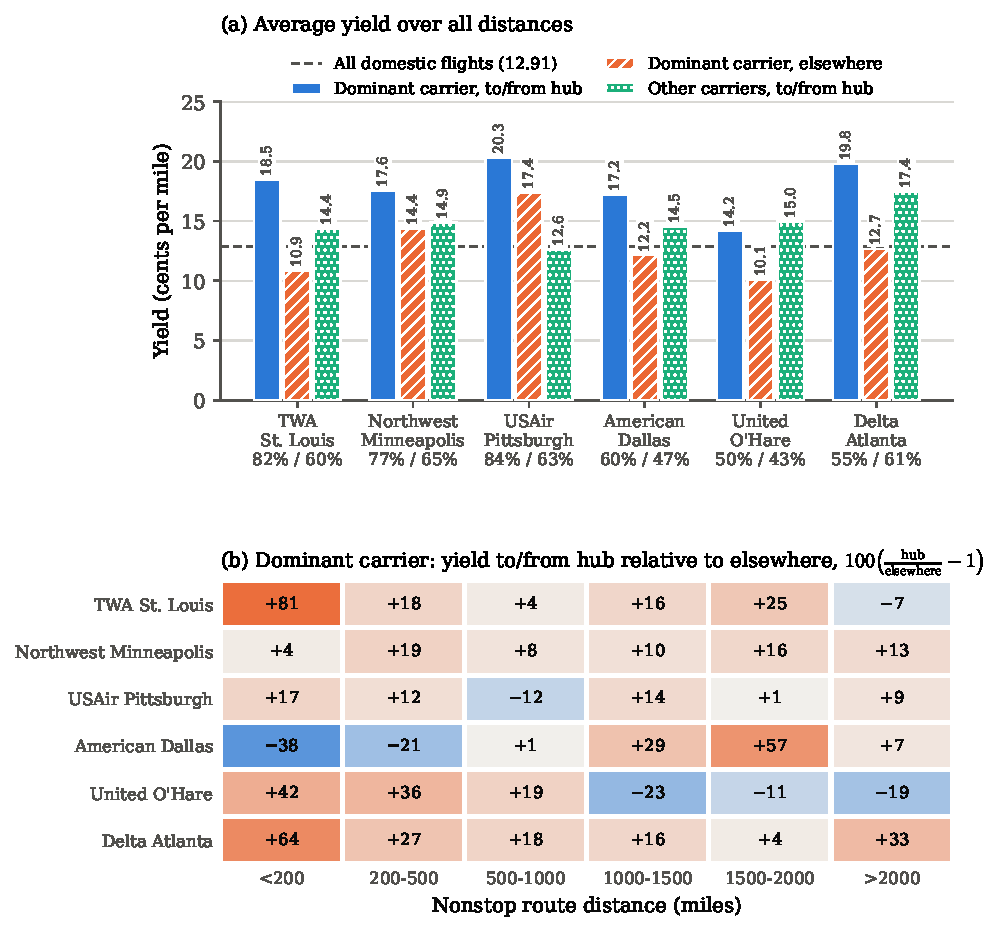
\includegraphics[width=0.97\linewidth]{figures/ch09/borenstein_yields.pdf}
\caption{Yields at six airports dominated by one carrier, third quarter of 1987. Panel (a) shows three yields
over all distances. They are the dominant carrier's yield on routes to or from its hub, its yield elsewhere in
its system, and the yield of other carriers on routes to or from the hub. The two percentages under each airport are the
dominant carrier's shares of enplanements and of originations there. Panel (b) shows, for each distance band,
the percentage by which the dominant carrier's yield to or from its hub exceeds its yield elsewhere. Yields fall
with distance, so panel (a) mixes fare levels with the distance composition of each group, while panel (b)
holds distance roughly fixed. Redrawn from \citet{Borenstein1989}, Table 1.}
\label{fig:09-bor-yields}
\end{figure}

Over all distances, the dominant carrier's yield at its hub exceeds its yield elsewhere at all six airports.
The gap ranges from 17\% for USAir at Pittsburgh ($\frac{20.32}{17.42} = 1.17$) to 70\% for TWA at St.\ Louis
($\frac{18.50}{10.86} = 1.70$). At five of the six airports, the dominant carrier's yield also exceeds that of
other carriers at the same airport. The exception is O'Hare, the least dominated airport in the table. There
United's yield of 14.19 cents falls short of the other carriers' 14.99 cents.

The comparison over all distances has a weakness. Yields fall steeply with distance, from 37.96 cents per mile
on routes under 200 miles to 7.16 cents on routes over 2,000 miles. A group that flies shorter routes therefore
shows a higher average yield even if it charges the same fare as others at each distance. Panel (b) of
\cref{fig:09-bor-yields} compares the dominant carrier with itself within distance bands. Its hub yield exceeds
its yield elsewhere in 29 of the 36 cells. The exceptions are Dallas on short routes ($-38\%$ and $-21\%$)
and O'Hare on routes over 1,000 miles ($-23\%$, $-11\%$ and $-19\%$). The others are Pittsburgh at 500 to
1,000 miles ($-12\%$) and St.\ Louis over 2,000 miles ($-7\%$). Against other carriers at the same airport, the dominant carrier has the
higher yield in 26 of the 35 cells with data. United at O'Hare is lower in five of six bands. USAir's 61\%
advantage over other carriers at Pittsburgh over all distances shrinks to between $-16\%$ and $+27\%$ within
bands, so most of it reflects the distance mix.\footnote{The within-band counts and percentages are our
calculations from Table 1 of the paper.}%

Borenstein argues that costs do not explain the hub premium (p.~356). Carriers have somewhat higher load
factors on flights to and from their hubs, which lowers cost per passenger. Passengers to or from a hub also
fly routes about as long as, or longer than, the carrier's other passengers. The higher cost per mile of short
flights therefore does not explain the gap either. The table cannot separate airport dominance from route
dominance, because a carrier that dominates an airport usually dominates the routes from it. The regressions
attempt this separation.

\subsection{The estimating equations}\label{sec:09-bor-equations}

\casehead{The pricing equation} Borenstein's first equation explains the log of a fare percentile by cost,
quality and market-structure variables. Let $P_{ft}$ denote one of FR20, FR50 or FR80 for carrier $f$ on route
$t$. Each percentile has its own regression with its own coefficients. In our notation, his equation (1), with
an error term $u_{ft}$ added, is
\begin{equation}\label{eq:09-bor-price}
\begin{aligned}
\ln P_{ft} = {} & a_f + b_D \ln \mathit{DISTANCE}_t + \gamma_1 \ln \mathit{LOADFAC}_{ft}
  + \gamma_2 \ln \mathit{EQUIP}_{ft} \\
& + \gamma_3 \ln \mathit{FREQ}_{ft} + \gamma_4 \ln \mathit{CIRC}_{ft} + \gamma_5\, \mathit{STOP}_{ft}
  + \gamma_6\, \mathit{PLANECHG}_{ft} \\
& + \phi_1\, \mathit{ORGSHARE}_{ft} + \phi_2\, \mathit{ORGHERF}_t + \phi_3\, \mathit{RUTSHARE}_{ft}
  + \phi_4\, \mathit{RUTHERF}_t \\
& + \phi_5 \ln \mathit{COMPCOST}_{ft} + \phi_6 \ln \mathit{TOURIST}_t
  + \sum_{k=1}^{24} \varrho_k\, \mathit{APT}_{kt} + u_{ft} .
\end{aligned}
\end{equation}
The coefficient letters group the variables by their hypothesized role (p.~349). The carrier effects $a_f$
capture carrier-wide differences in cost and reputation. Distance, with coefficient $b_D$, primarily affects
production cost. The six $\gamma$ variables affect both cost and service quality, so their signs are ambiguous
in advance. The six $\phi$ variables primarily indicate market power. The 24 coefficients $\varrho_k$ measure
scarcity rents at airports that may be congested. \Cref{tab:09-bor-vars} defines each variable and gives the
sign that Borenstein expects.

\begin{table}[htbp]
\centering
\caption{Variables of the pricing equation}
\label{tab:09-bor-vars}
\footnotesize
\renewcommand{\arraystretch}{1.12}
\begin{tabularx}{\linewidth}{@{}l >{\raggedright\arraybackslash}X l c@{}}
\toprule
Variable & Definition and construction & Group & Sign \\
\midrule
FR20, FR50, FR80 & Percentiles of the passenger-weighted distribution of the fares paid to the carrier on the
route. A round trip counts as two trips at half fare. & dependent & \\
DISTANCE & Nonstop mileage between the endpoints ($d_t$ in \cref{sec:09-data}). & cost & $+$ \\
LOADFAC & Load factor of the segments used by the carrier's passengers on the route, averaged over the
segments of an itinerary by distance and over itineraries by passengers. & cost, quality & ? \\
EQUIP & Seats per plane, averaged in the same way. & cost, quality & ? \\
FREQ & Minimum number of flights in the quarter on any segment of an itinerary, averaged over itineraries by
passengers. & cost, quality & ? \\
CIRC & Average total routing mileage of the carrier's passengers (TOTMILE) divided by DISTANCE. & cost, quality
& ? \\
STOP & Average number of on-plane stops per passenger. & cost, quality & ? \\
PLANECHG & Average number of changes of plane per passenger. & cost, quality & ? \\
ORGSHARE & Carrier's share of passenger originations at the two endpoints, averaged with weights equal to the
shares of the route's travelers whose tickets originate at each endpoint. & market power & $+$ \\
ORGHERF & Herfindahl index of originations at the two endpoints, averaged with the same weights. & market power
& ? \\
RUTSHARE & Carrier's share of the route's local passengers. & market power & $+$ \\
RUTHERF & Herfindahl index of the route's local passengers. & market power & ? \\
COMPCOST & Average standardized cost per available seat-mile of the other carriers on the route, weighted by
their route shares. & market power & $+$ \\
TOURIST & Tourism index (hotel income from group and tourist customers over personal income) of each endpoint,
weighted by the share of travelers who originate at the other endpoint. & market power & $-$ \\
APT$_k$ & Indicator that airport $k$ is an endpoint, divided by DISTANCE in thousands of miles. & scarcity &
$+$ \\
\bottomrule
\end{tabularx}

\smallskip
\begin{minipage}{\linewidth}
\footnotesize Notes: ``Group'' is the role that Borenstein assigns to each variable and ``Sign'' the sign he
expects, with ? for an ambiguous sign. Load factor, equipment, frequency and stops come from the Service
Segment Data, fares, shares and circuity from the DB1A sample, and enplanements from the Nonstop Market Data.
Source: \citet{Borenstein1989}, pp.~349--351 and Appendix.
\end{minipage}
\end{table}

\casehead{Constructed variables} Several variables are averages over the two endpoints $e \in \{1,2\}$ of the
route. Let $\varpi_{te}$ be the share of the route's travelers whose tickets originate at endpoint $e$. Let
$o_{fe}$ be carrier $f$'s share of all passenger originations at airport $e$, and let $\mathit{TRIX}_e$ be the
tourism index of the metropolitan area of $e$. Then
\begin{equation}\label{eq:09-bor-org}
\begin{gathered}
\mathit{ORGSHARE}_{ft} = \sum_{e=1}^{2} \varpi_{te}\, o_{fe}, \qquad
\mathit{ORGHERF}_t = \sum_{e=1}^{2} \varpi_{te} \sum_{k} o_{ke}^2, \\
\mathit{TOURIST}_t = \varpi_{t1}\, \mathit{TRIX}_2 + \varpi_{t2}\, \mathit{TRIX}_1 .
\end{gathered}
\end{equation}
The tourism measure weights each endpoint by the share of travelers who start at the other end, so it measures
the tourist appeal of the route's destinations. Origination shares exclude connecting passengers. Borenstein
reports that measures based on enplanements, which include them, give very similar results (p.~349).

The cost of rivals enters through
\begin{equation}\label{eq:09-bor-compcost}
\mathit{COMPCOST}_{ft} = \sum_{k \neq f} \frac{s_{kt}}{1 - s_{ft}}\, \mathit{COST}_k ,
\end{equation}
where $s_{kt}$ is carrier $k$'s route share, so that $s_{ft} = \mathit{RUTSHARE}_{ft}$. $\mathit{COST}_k$ is a
standardized cost per available seat-mile. To construct it, Borenstein regresses cost per available seat-mile on
a constant and average length of haul across the 17 carriers with data. He then adds each carrier's residual to
0.08, roughly the average cost of a carrier with the mean length of haul (p.~363). Small carriers without data
receive 0.08. COMPCOST proxies for the competitiveness of rivals, whose prices are endogenous and whose service
data are incomplete (p.~351).

Finally, the scarcity variables are
\begin{equation}\label{eq:09-bor-apt}
\mathit{APT}_{kt} = \frac{1000 \cdot \indic\{k \text{ is an endpoint of } t\}}{\mathit{DISTANCE}_t} ,
\end{equation}
for 24 airports (p.~351). They are the 22 airports that the Federal Aviation Administration monitored for
congestion and the airports of Orange County and Long Beach, which faced strict local limits on takeoffs and
landings. Four of the monitored airports allocated slots: O'Hare, Kennedy, La Guardia and Washington National.

\casehead{Expected signs} The $\gamma$ variables move cost and quality in directions that push price opposite
ways (pp.~349--350). A higher load factor lowers cost per passenger, which lowers fares. Full flights also tend
to operate at peak times, when the opportunity cost of aircraft is high, which raises fares. Crowded planes,
finally, lower service quality and reservation prices. Larger aircraft have a lower cost per seat-mile on
flights over 500 miles. They are also more comfortable and thought to be safer, which raises demand. Frequent
service lowers cost per flight, because aircraft on dense routes fly more hours per day. It also lowers the
frequency delay of \cref{sec:09-regulation}, the gap between a traveler's preferred departure time and the
nearest flight \citep{DouglasMiller1974}. Frequency delay matters most to travelers with high time values, who pay the high
fares. Circuity, stops and changes of plane raise cost, by lengthening routings or shortening average hauls,
and they lower quality.

Among the $\phi$ variables, Borenstein expects ORGSHARE, RUTSHARE and COMPCOST to raise fares and TOURIST to
lower them (pp.~350--351). The concentration measures have ambiguous signs, and their interpretation drives the
paper. Holding the carrier's own route share fixed, a higher RUTHERF means that the traffic the carrier does not
carry is more concentrated. If a dominant carrier's high price creates an umbrella, this raises the observed
carrier's price, so $\phi_4 > 0$. If a dominant carrier instead has a competitive advantage through marketing
devices, it may lower the profit-maximizing price of its rivals, so $\phi_4 < 0$. Endpoint concentration is
ambiguous for a related reason. A carrier may prefer many small rivals at its airports to one large rival,
while coordination, such as an agreement not to enter one another's routes, is easier among few firms.

\casehead{Functional form} A firm with market power sets price equal to marginal cost times a markup that
depends on the elasticity of the demand it faces. Logs turn this product into a sum, and earlier studies used
the same multiplicative form \citep{GrahamKaplanSibley1983,BaileyGrahamKaplan1985}. Most variables therefore
enter in logs, with constant elasticities. \Cref{sec:09-pricing-conduct} derives this specification from a
model of conduct. Let collusiveness rise with concentration as $\eta_t = \eta_0 + \eta_1 \HHI_t$, and let the
elasticity be a common $\varepsilon$. Because the equation omits the interaction $\HHI_t s_{ft}$ of
\cref{eq:09-umbrella}, the route-share coefficient is then $\phi_3 \approx \frac{1 - \eta_0 - \eta_1 \bar H}{\varepsilon}$
and the route-Herfindahl coefficient is $\phi_4 \approx \frac{\eta_1 (1 - \bar s)}{\varepsilon}$. Here $\bar H$
and $\bar s$ are the sample means of RUTHERF and RUTSHARE. The cost and quality variables parametrize
$\ln mc_{ft}$, and the constant terms are absorbed by the carrier effects.

The theory thus implies that shares enter linearly, and Borenstein gives a direct argument for the same choice
(p.~354). A log specification would give a rise in share from 1\% to 2\% the same effect as a rise from 30\% to
60\%, which is implausible. ORGSHARE enters linearly for the same reason, and
the two Herfindahl indices enter linearly for ease of comparison. The signs and approximate significance of
the estimates are robust to logs for each of these variables. STOP and PLANECHG also enter linearly, so each
stop or change of plane has the same proportional effect on price.

\Cref{rem:09-share-coef} shows that a Cournot reading of the 2SLS share coefficients ($\bar\eta = 0$, so
$\varepsilon = \frac{1}{\phi_3}$) would require route elasticities of $\frac{1}{0.1120} = 8.9$,
$\frac{1}{0.0288} = 34.7$ and $\frac{1}{0.2238} = 4.5$ for the three percentiles. The variation across
percentiles adds a further difficulty. A homogeneous-goods model has one price per route, and hence one
elasticity for all fares, while the share coefficients differ nearly eightfold across percentiles. Each
percentile behaves as if it faced its own demand. A model with differentiated products and heterogeneous
travelers delivers this pattern (\cref{sec:09-pricing-types}).

The scarcity terms need a different treatment (p.~354). A scarcity rent should add the same dollar amount to
every fare from an airport, whatever the route. Suppose the fare is $P_{ft} = P^0_{ft} + R_k$, where $P^0_{ft}$
is the fare without the rent and $R_k$ is the rent at endpoint $k$. Taking logs and using
$\ln(1 + x) \approx x$ for small $x$,
\begin{align*}
\ln P_{ft} &= \ln P^0_{ft} + \ln\left(1 + \frac{R_k}{P^0_{ft}}\right) \\
&\approx \ln P^0_{ft} + \frac{R_k}{P^0_{ft}} .
\end{align*}
If the rent-free fare is proportional to distance, $P^0_{ft} = c\, \mathit{DISTANCE}_t$, the last term becomes
\begin{equation*}
\frac{R_k}{c\, \mathit{DISTANCE}_t} = \frac{R_k}{1000\, c} \cdot \frac{1000}{\mathit{DISTANCE}_t}
= \varrho_k\, \mathit{APT}_{kt}, \qquad \text{with } \varrho_k = \frac{R_k}{1000\, c} .
\end{equation*}
The coefficient $\varrho_k$ is thus the rent as a fraction of the fare on a 1,000-mile route. A plain indicator
would instead make the rent proportional to the fare and assign larger rents to longer routes. Estimating the
additive form directly would require iterative nonlinear methods, which would have been difficult with his
number of observations and variables. Borenstein therefore calls the distance scaling a partial solution. Fares
rise less than proportionally with distance ($b_D$ lies between 0.33 and 0.41 in \cref{tab:09-bor-main}), so
dividing by distance overcorrects somewhat.

\casehead{The relative-price equation} The second equation compares two carriers on the same route. Add to
\cref{eq:09-bor-price} a route effect $\Upsilon_t$ that collects every determinant of fares common to all carriers
on route $t$, observed or not. Collect the variables that vary across carriers on a route in the row vector
\begin{equation*}
z_{ft} = \big(\ln \mathit{LOADFAC}_{ft}, \ln \mathit{EQUIP}_{ft}, \ln \mathit{FREQ}_{ft}, \ln \mathit{CIRC}_{ft},
\mathit{STOP}_{ft}, \mathit{PLANECHG}_{ft}\big),
\end{equation*}
with coefficients $\gamma = (\gamma_1, \dots, \gamma_6)^\top$. The pricing equation becomes
\begin{equation*}
\ln P_{ft} = a_f + \Upsilon_t + z_{ft}\gamma + \phi_1\, \mathit{ORGSHARE}_{ft} + \phi_3\, \mathit{RUTSHARE}_{ft}
+ \phi_5 \ln \mathit{COMPCOST}_{ft} + u_{ft} .
\end{equation*}
Here $\Upsilon_t$ absorbs distance, the two Herfindahl indices, the tourism index, the scarcity terms and any
unobserved demand or cost shifter at the route level. Write this equation for carriers $a$ and $b$ on route $t$
and subtract. The route effect cancels because $\Upsilon_t - \Upsilon_t = 0$. Borenstein also omits the difference in
COMPCOST (p.~355, n.~35). Its role in the pricing equation was to proxy for the other carriers on the route. In
the relative-price equation one rival enters directly and the remaining rivals are common to both carriers. The
result is his equation (4):
\begin{equation}\label{eq:09-bor-rel}
\begin{aligned}
\ln P_{at} - \ln P_{bt} = {} & a_a - a_b + \gamma_1 (\ln \mathit{LOADFAC}_{at} - \ln \mathit{LOADFAC}_{bt}) \\
& + \gamma_2 (\ln \mathit{EQUIP}_{at} - \ln \mathit{EQUIP}_{bt})
  + \gamma_3 (\ln \mathit{FREQ}_{at} - \ln \mathit{FREQ}_{bt}) \\
& + \gamma_4 (\ln \mathit{CIRC}_{at} - \ln \mathit{CIRC}_{bt})
  + \gamma_5 (\mathit{STOP}_{at} - \mathit{STOP}_{bt}) \\
& + \gamma_6 (\mathit{PLANECHG}_{at} - \mathit{PLANECHG}_{bt})
  + \phi_1 (\mathit{ORGSHARE}_{at} - \mathit{ORGSHARE}_{bt}) \\
& + \phi_3 (\mathit{RUTSHARE}_{at} - \mathit{RUTSHARE}_{bt}) + u_{at} - u_{bt} .
\end{aligned}
\end{equation}
The coefficients are those of \cref{eq:09-bor-price}. The two carriers are drawn at random among those that meet
the sample criteria (p.~355). The carrier effects enter as the difference $a_a - a_b$, which a regression
implements with indicators equal to $+1$ for carrier $a$ and $-1$ for carrier $b$.

Differencing has a benefit and a cost. The benefit is that every unobserved route-level shifter of demand or
cost drops out. The estimates of $\phi_1$ and $\phi_3$ then no longer rely on the route controls of
\cref{eq:09-bor-price}. The cost is that the coefficients on route-level market structure, $\phi_2$ and
$\phi_4$, are no longer identified. The equation answers a narrower question, which is the one the asymmetry
hypothesis poses. Does the carrier with the larger share of a route, or of its endpoints, charge more than its
rival on the same route? Under a complete umbrella with a homogeneous product, $\eta_t = 1$ and every carrier on
the route has conduct $\theta_{ft} = 1$. The share term in \cref{eq:09-pricing-approx} then vanishes, and all
carriers charge the same markup, so $\phi_3 = 0$ in \cref{eq:09-bor-rel}. Under the differentiated-products
model of \cref{prop:09-dominance}, the relative price instead rises with the share gap. Let $s$ be a common
share of all potential travelers, $L$ the Lerner index there and $s_0$ the outside share. \Cref{cor:09-relprice}
gives a slope of $\frac{L}{1-s}$ in these shares, or $\frac{L(1-s_0)}{1-s}$ in route shares. The latter is
the structural counterpart of $\phi_3$ in \cref{eq:09-bor-rel}.

\subsection{Estimation and identification}\label{sec:09-bor-ident}

\casehead{Why least squares fails} A carrier's route share depends on its own price. To see the consequence,
add a share equation to the pricing equation and solve the two jointly. Suppress the other regressors, which
we take as exogenous, and write
\begin{align*}
\ln P_{ft} &= \phi_3\, s_{ft} + u_{ft}, \\
s_{ft} &= \Psi_{ft} - b_s \ln P_{ft} + v_{ft} .
\end{align*}
Here $s_{ft} = \mathit{RUTSHARE}_{ft}$, $\Psi_{ft}$ collects exogenous shifters of the share, $b_s > 0$
measures how fast the share falls with the carrier's own price, and $v_{ft}$ is an unobserved demand shifter.
Substitute the first equation into the second:
\begin{equation*}
s_{ft} = \Psi_{ft} - b_s \phi_3\, s_{ft} - b_s u_{ft} + v_{ft} .
\end{equation*}
Collect the terms in $s_{ft}$ and solve, assuming $1 + b_s \phi_3 > 0$:
\begin{equation*}
s_{ft} = \frac{\Psi_{ft} - b_s u_{ft} + v_{ft}}{1 + b_s \phi_3} .
\end{equation*}
Let $\Var(u_{ft}) = \sigma_u^2$ and $\Cov(u_{ft}, v_{ft}) = \sigma_{uv}$, and let $\Psi_{ft}$ be uncorrelated
with both errors. The ordinary least squares (OLS) estimator then has probability limit
\begin{equation}\label{eq:09-bor-olsbias}
\plim \hat\phi_3^{\mathrm{OLS}} = \phi_3 + \frac{\Cov(s_{ft}, u_{ft})}{\Var(s_{ft})}
= \phi_3 + \frac{\sigma_{uv} - b_s \sigma_u^2}{(1 + b_s\phi_3) \Var(s_{ft})} .
\end{equation}
With other regressors present, $\Var(s_{ft})$ is the variance of the share after projection on them. Two forces
compete. The simultaneity term $-b_s\sigma_u^2$ biases the estimate down. A carrier hit by a positive cost
or pricing shock charges more and loses passengers, so high prices go with low shares. The term $\sigma_{uv}$
biases the estimate up if unobserved quality raises both the share and the price, which is the efficiency
argument of \citet{Demsetz1973} in airline form. A Hausman test (described below) rejects the exogeneity of
RUTSHARE and RUTHERF (p.~352), so the preferred estimates use instruments.

\casehead{The instrument for route share} An instrument must shift a carrier's route share without entering its
pricing equation. Measures of rivals' presence at the endpoint airports come to mind. The airport dominance
effects of \cref{sec:09-dominance-sources}, however, make such measures candidates for the pricing equation
itself (p.~352). Borenstein resolves the problem with an asymmetry. The marketing advantages of airport
dominance do not require large operations at both ends of a route. Entry onto a route, in contrast, benefits
from presence at both ends. The excluded instrument is the carrier's share of the geometric means of endpoint
enplanements,
\begin{equation}\label{eq:09-genpsh}
\mathit{GENPSH}_{ft} = \frac{\sqrt{\mathit{ENP}_{f1}\, \mathit{ENP}_{f2}}}
{\sum_{k} \sqrt{\mathit{ENP}_{k1}\, \mathit{ENP}_{k2}}} ,
\end{equation}
which is his equation (2). Here $\mathit{ENP}_{k1}$ and $\mathit{ENP}_{k2}$ are carrier $k$'s average daily
enplanements at the two endpoints of route $t$ during the quarter, and the sum runs over all carriers
(p.~352).

The geometric mean gives the instrument its content. It is zero when a carrier has no enplanements at one of
the endpoints. For a given total $\mathit{ENP}_{f1} + \mathit{ENP}_{f2}$, it is largest when the two are equal.
GENPSH therefore rewards balanced presence at both ends. ORGSHARE, which appears in the pricing equation,
averages the carrier's endpoint shares linearly. A carrier with a large share at one end and a small share at
the other can have a high ORGSHARE but a low GENPSH. Conditional on ORGSHARE, GENPSH thus varies with the
balance of the carrier's presence across the endpoints. It also varies with connecting operations, since
enplanements count connecting passengers and originations do not. Borenstein chooses enplanements because they
better measure a carrier's investment in physical capital and long-term labor contracts at an airport
(p.~352, n.~30).

Two pieces of evidence support relevance. The first comes from \citet{Berry1992}, which Borenstein cites as a
1989 working paper (p.~352, n.~29). Berry starts from the 1,225 possible city pairs among the 50 largest U.S.
cities \citep[p.~903]{Berry1992}. He drops 6 pairs that have no listings in the Origin and Destination Survey,
which leaves 1,219 markets \citep[p.~903, n.~9, and p.~904]{Berry1992}. He measures entry between the first and the third quarter of 1980
\citep[p.~904]{Berry1992}. Of the 3,590
potential entrants that already served both cities of a pair, 6.46\% entered it. Of those that served one city,
0.36\% entered, a rate about 18 times lower. Only 4 of the 47,600 potential entrants that served neither city entered,
a rate of 0.01\% \citep[Table~III]{Berry1992}. The second piece of evidence is Borenstein's own. In the first
stage of the estimation, both ORGSHARE and GENPSH are highly significant (p.~352). The paper does not report the first-stage coefficients or $F$ statistics.

The exclusion restriction requires that GENPSH affect fares only through route share. Borenstein states the
condition plainly. It is valid if a carrier's current prices respond to actual competition but not to threats
of entry (p.~352). He defends it on timing grounds. An incumbent can change its fares much faster than a rival
can move from announcing entry to flying. It therefore need not price against potential entrants in advance. The USAir testimony quoted in \cref{sec:09-contest-fail} supports this view.

If the restriction fails, the bias has a predictable sign. Potential entrants with large operations at both
endpoints raise the denominator of \cref{eq:09-genpsh}, so a carrier's GENPSH is low exactly when such entrants
are present. Suppose a carrier that faces well-placed potential entrants holds its fares down to deter entry, a
practice called \emph{limit pricing}. Its fares then rise with GENPSH at a given route share, and the true
equation contains a term $\phi_G\, \mathit{GENPSH}_{ft}$ with $\phi_G > 0$. Ignore RUTHERF for the moment, write $g_{ft} = \mathit{GENPSH}_{ft}$, and let a tilde denote the
residual after projection on the included exogenous regressors. The IV estimator has probability limit
\begin{align}
\plim \hat\phi_3^{\mathrm{IV}} &= \frac{\Cov(\tilde g_{ft}, \ln P_{ft})}{\Cov(\tilde g_{ft}, \tilde s_{ft})}
\notag \\
&= \frac{\phi_3 \Cov(\tilde g_{ft}, \tilde s_{ft}) + \phi_G \Var(\tilde g_{ft})}{\Cov(\tilde g_{ft}, \tilde s_{ft})}
\notag \\
&= \phi_3 + \frac{\phi_G}{\pi_1} . \label{eq:09-bor-ivbias}
\end{align}
The second line substitutes the true equation and uses $\Cov(\tilde g_{ft}, u_{ft}) = 0$. In the third line,
$\pi_1 = \frac{\Cov(\tilde g_{ft}, \tilde s_{ft})}{\Var(\tilde g_{ft})}$ is the first-stage coefficient on
GENPSH. Since $\pi_1 > 0$ and $\phi_G > 0$, limit pricing against potential entrants biases the estimated
share effect upward. A violation of this kind would make Borenstein's estimates of $\phi_3$ too large. The
POTCOMP specification below offers a check. Controlling for potential competitors should absorb part of this
bias and lower the route-share coefficients. Instead they rise slightly (Panel B of \cref{tab:09-bor-main}),
which suggests that the bias is small.

\casehead{Potential competition} Borenstein addresses the exclusion restriction in a second way, by measuring
potential competition directly (pp.~352--353). The variable
\begin{equation}\label{eq:09-bor-potcomp}
\mathit{POTCOMP}_{ft} = \frac{\sum_{k \in \mathcal{P}_t} \sqrt{\mathit{ENP}_{k1}\, \mathit{ENP}_{k2}}}
{\sum_{k} \sqrt{\mathit{ENP}_{k1}\, \mathit{ENP}_{k2}}}
\end{equation}
has the construction of GENPSH, but its numerator sums over the set $\mathcal{P}_t$ of carriers with less than
1\% of the route's traffic (p.~364). These carriers are present at the endpoints but not yet significant on the
route. In an alternative specification POTCOMP enters \cref{eq:09-bor-price} directly, while GENPSH still
instruments route share. POTCOMP may itself be endogenous. High fares on a route attract entry, which turns
potential competitors into actual ones and lowers POTCOMP. A positive shock $u_{ft}$ therefore goes with a low
POTCOMP, which biases its coefficient toward a negative value (p.~359, n.~44).

\casehead{The instrument for route concentration} The route Herfindahl index contains the square of the
carrier's own share, so it is endogenous whenever RUTSHARE is. Borenstein constructs an instrument by
decomposing the index (p.~353). Write $s_{ft}$ for the carrier's share and $\HHI_t = \mathit{RUTHERF}_t$. Split
the sum of squared shares into the carrier's own term and its rivals' terms:
\begin{align*}
\HHI_t &= s_{ft}^2 + \sum_{k \neq f} s_{kt}^2 \\
&= s_{ft}^2 + (1 - s_{ft})^2 \sum_{k \neq f} \left(\frac{s_{kt}}{1 - s_{ft}}\right)^2 \\
&= s_{ft}^2 + (1 - s_{ft})^2 H_{-f,t} .
\end{align*}
Here $H_{-f,t}$ is the Herfindahl index of the traffic that carrier $f$ does not carry, computed from each
rival's share of that traffic. Solving the last line for $H_{-f,t}$ expresses it in observed variables:
\begin{equation*}
H_{-f,t} = \frac{\mathit{RUTHERF}_t - \mathit{RUTSHARE}_{ft}^2}{(1 - \mathit{RUTSHARE}_{ft})^2} .
\end{equation*}

The instrument rests on two assumptions. (a) GENPSH is a valid instrument for RUTSHARE. (b) The division among
rivals of the traffic that carrier $f$ does not carry is exogenous to $f$'s price. In Borenstein's example,
TWA's price on the Boston to Los Angeles route does not affect how the passengers it does not get divide between
American and United. Under (b), $H_{-f,t}$ is exogenous. Replace the own share by its fitted value
$\widehat{\mathit{RUTSHARE}}_{ft}$ from the first-stage regression on all exogenous variables:
\begin{equation}\label{eq:09-irutherf}
\mathit{IRUTHERF}_{ft} = \widehat{\mathit{RUTSHARE}}_{ft}^{\,2}
+ \frac{\mathit{RUTHERF}_t - \mathit{RUTSHARE}_{ft}^2}{(1 - \mathit{RUTSHARE}_{ft})^2}
\big(1 - \widehat{\mathit{RUTSHARE}}_{ft}\big)^2 .
\end{equation}
This is Borenstein's equation (3). In the constructed index, each rival's share becomes
$s_{kt} \frac{1 - \widehat{\mathit{RUTSHARE}}_{ft}}{1 - s_{ft}}$. The rescaling leaves the Herfindahl index of the
traffic not carried by $f$ equal to $H_{-f,t}$, as Borenstein notes. IRUTHERF then serves as the excluded
instrument for RUTHERF. The same assumption (b) is needed for COMPCOST, whose weights in
\cref{eq:09-bor-compcost} are the rivals' shares of the traffic that $f$ does not carry (p.~353).

\begin{remark}[When is assumption (b) plausible?]\label{rem:09-bor-iia}
Assumption (b) holds exactly in a logit model of route demand, holding rivals' prices fixed. Route shares are
shares of the route's passengers, so the outside good drops out and
$s_{kt} = \frac{e^{\delta_{kt}}}{\sum_{j} e^{\delta_{jt}}}$, with the sum over the carriers on the route. Then
\begin{equation*}
\frac{s_{kt}}{1 - s_{ft}} = \frac{e^{\delta_{kt}}}{\sum_{j \neq f} e^{\delta_{jt}}} ,
\end{equation*}
which involves neither $\delta_{ft}$ nor $p_{ft}$. This is the independence of irrelevant alternatives of
\cref{ch:logit}. The assumption fails when some rivals are closer substitutes for $f$ than others, for example
when one rival shares $f$'s hub airport. It can also fail in equilibrium, since rivals adjust their prices when
$f$ changes its own.
\end{remark}

\begin{remark}[A constructed instrument]\label{rem:09-bor-generated}
IRUTHERF is a nonlinear function of first-stage fitted values. Substituting such a function for RUTHERF in the
second stage would not in general give consistent estimates, because the first-stage residual does not drop out
of a nonlinear function. Borenstein instead uses IRUTHERF as an excluded instrument in the first-stage regression
for RUTHERF. Any function of exogenous variables is a valid instrument, so this use is consistent under (a) and
(b). The nonlinearity affects only how strongly IRUTHERF predicts RUTHERF.
\end{remark}

\casehead{Load factor and the Hausman test} Load factor may also be endogenous, since a low fare fills planes.
Borenstein instruments it with LOADPOP, the passenger-weighted average over itineraries of the summed
populations of all cities where the traveler is on the ground, including stops and connections (pp.~353, 363).
The idea is that populous cities along an itinerary add traffic to its segments and so raise load factors. A
Hausman test does not reject exogeneity of LOADFAC at any reasonable significance level, so the reported
estimates treat it as exogenous (pp.~356--357).

The Hausman test compares two estimators \citep{Hausman1978}. Under the null hypothesis that the suspect
regressors are exogenous, OLS is consistent and efficient, while 2SLS is consistent but less precise. Under the
alternative only 2SLS is consistent. Let $\hat\vartheta_S$ collect the estimated coefficients on the suspect
regressors and $\hat V$ their estimated variance matrix. The statistic
\begin{equation}\label{eq:09-bor-hausman}
\mathcal{H} = \big(\hat\vartheta_S^{\mathrm{2SLS}} - \hat\vartheta_S^{\mathrm{OLS}}\big)^\top
\big[\hat V^{\mathrm{2SLS}} - \hat V^{\mathrm{OLS}}\big]^{-1}
\big(\hat\vartheta_S^{\mathrm{2SLS}} - \hat\vartheta_S^{\mathrm{OLS}}\big)
\end{equation}
is asymptotically $\chi^2$ under the null, with degrees of freedom equal to the number of suspect regressors
(\cref{sec:A-spectests}). A large value rejects exogeneity. For RUTSHARE and RUTHERF the test rejects, and
for LOADFAC it does not.

Treating LOADFAC as endogenous anyway raises the estimated ORGSHARE effects somewhat and raises all standard
errors (p.~357, n.~38). The LOADFAC coefficient itself becomes much more negative and much less precise
(p.~358, n.~40). Simultaneity predicts the opposite movement. Low fares raise load factors, which pushes the
least-squares coefficient down, so a correction should make it less negative.

\casehead{Variables without instruments} A carrier's choices of nonstop versus connecting service, aircraft
size, frequency, stops, changes of plane and circuity are part of its network design. They may respond to the
same shocks as its fares (p.~353). Even LOADPOP is open to doubt, since the populations are exogenous but their
summation by itinerary depends on routing choices. For lack of instruments, Borenstein treats these variables as
exogenous and interprets their coefficients with possible biases in mind.

\casehead{Pooling and the error structure} A test rejects a common constant across carriers, so the equation
includes carrier fixed effects $a_f$ (pp.~353--354). A further test of common slopes across carriers does not
reject pooling at conventional levels, so all other coefficients are common to the nine carriers. The
scarcity coefficients $\varrho_k$ are common by construction, since a scarcity rent is the same for every
carrier at an airport. The same tests applied to \cref{eq:09-bor-rel} again do not reject pooling (p.~355).
Keeping one carrier per route gives up information to secure independent errors. A modern study would keep
every qualifying carrier and cluster the standard errors by route (\cref{sec:A-cluster}).

\casehead{The estimator} The preferred estimates are 2SLS with asymptotic standard errors. The procedure has
three steps. First, regress RUTSHARE on GENPSH and all included exogenous regressors, and keep the fitted
values. Second, construct IRUTHERF from \cref{eq:09-irutherf}. Third, estimate \cref{eq:09-bor-price} by 2SLS,
treating RUTSHARE and RUTHERF as endogenous, with GENPSH and IRUTHERF as excluded instruments. With two
endogenous regressors and two excluded instruments, the equation is exactly identified. Let $X_{ft}$ be the row
of regressors, let $Z_{ft}$ be the same row with GENPSH and IRUTHERF in place of RUTSHARE and RUTHERF, and let
$\vartheta$ be the coefficient vector. The estimator solves the sample analogue of
$\E[Z_{ft}^\top u_{ft}] = 0$,
\begin{equation*}
\hat\vartheta = \Big(\sum_{t} Z_{ft}^\top X_{ft}\Big)^{-1} \sum_{t} Z_{ft}^\top \ln P_{ft} ,
\end{equation*}
where each route $t$ contributes the one carrier $f$ selected for it. The paper treats the endogeneity in
\cref{eq:09-bor-rel} in the same way, without detailing the instrument for the share difference. OLS estimates
are reported for comparison.

\subsection{Results}\label{sec:09-bor-results}

\casehead{The pricing equation} \Cref{tab:09-bor-main} reproduces Table 2 of the paper. Panel A gives the 2SLS
estimates of \cref{eq:09-bor-price} for the three fare percentiles. Panel B gives the market-power coefficients
from two alternative specifications, one with POTCOMP added and one estimated by OLS. The paper summarizes the
carrier effects and the scarcity coefficients in the text without reporting them. \Cref{fig:09-bor-coefs} plots
the main market-power coefficients with 95\% confidence intervals.

\begin{table}[htbp]
\centering
\caption{The pricing equation: estimates of \cref{eq:09-bor-price}}
\label{tab:09-bor-main}
\footnotesize
\begin{tabular}{@{}lccc@{}}
\toprule
\multicolumn{4}{@{}l}{\textit{Panel A. 2SLS}} \\
\addlinespace
Dependent variable & $\ln$ FR20 & $\ln$ FR50 & $\ln$ FR80 \\
\midrule
$\ln$ DISTANCE & 0.4138$^{*}$ & 0.3348$^{*}$ & 0.3559$^{*}$ \\
 & (0.0103) & (0.0124) & (0.0133) \\
$\ln$ LOADFAC & $-0.0754^{*}$ & $-0.0425$ & $-0.0240$ \\
 & (0.0264) & (0.0318) & (0.0341) \\
$\ln$ EQUIP & $-0.0160$ & $-0.0050$ & $-0.0691^{*}$ \\
 & (0.0187) & (0.0225) & (0.0242) \\
$\ln$ FREQ & 0.0140$^{\#}$ & 0.0236$^{*}$ & 0.0428$^{*}$ \\
 & (0.0078) & (0.0094) & (0.0101) \\
$\ln$ CIRC & 0.1458$^{*}$ & 0.1272$^{*}$ & 0.2062$^{*}$ \\
 & (0.0412) & (0.0497) & (0.0533) \\
STOP & $-0.0470$ & $-0.0340$ & $-0.1327^{*}$ \\
 & (0.0292) & (0.0352) & (0.0377) \\
PLANECHG & $-0.0293^{*}$ & $-0.0776^{*}$ & $-0.0616^{*}$ \\
 & (0.0111) & (0.0134) & (0.0144) \\
ORGSHARE & 0.0345 & 0.1254$^{\#}$ & 0.1191$^{\#}$ \\
 & (0.0549) & (0.0661) & (0.0710) \\
ORGHERF & $-0.0699$ & $-0.0893$ & 0.0766 \\
 & (0.0623) & (0.0751) & (0.0806) \\
RUTSHARE & 0.1120$^{\#}$ & 0.0288 & 0.2238$^{*}$ \\
 & (0.0606) & (0.0731) & (0.0784) \\
RUTHERF & 0.1559$^{\dagger}$ & 0.1822$^{\dagger}$ & $-0.1787^{\dagger}$ \\
 & (0.0696) & (0.0839) & (0.0901) \\
$\ln$ COMPCOST & 0.5042$^{*}$ & 0.7010$^{*}$ & 0.8374$^{*}$ \\
 & (0.0453) & (0.0546) & (0.0586) \\
$\ln$ TOURIST & $-0.0187^{*}$ & $-0.0558^{*}$ & $-0.0991^{*}$ \\
 & (0.0058) & (0.0070) & (0.0076) \\
\addlinespace
$R^2$ & 0.683 & 0.494 & 0.508 \\
Observations & 3,591 & 3,591 & 3,591 \\
\bottomrule
\end{tabular}

\bigskip
\begin{tabular}{@{}lcccccc@{}}
\toprule
\multicolumn{7}{@{}l}{\textit{Panel B. Market-power coefficients in alternative specifications}} \\
\addlinespace
& \multicolumn{3}{c}{2SLS with POTCOMP} & \multicolumn{3}{c}{OLS} \\
\cmidrule(lr){2-4} \cmidrule(l){5-7}
Dependent variable & $\ln$ FR20 & $\ln$ FR50 & $\ln$ FR80 & $\ln$ FR20 & $\ln$ FR50 & $\ln$ FR80 \\
\midrule
ORGSHARE & 0.0365 & 0.1227$^{\#}$ & 0.1205$^{\#}$ & 0.0819$^{\#}$ & 0.1229$^{*}$ & 0.1228$^{\dagger}$ \\
 & (0.0536) & (0.0647) & (0.0696) & (0.0426) & (0.0514) & (0.0551) \\
ORGHERF & $-0.0684$ & $-0.0750$ & 0.0934 & $-0.0264$ & $-0.0660$ & $-0.0033$ \\
 & (0.0633) & (0.0764) & (0.0822) & (0.0543) & (0.0656) & (0.0702) \\
RUTSHARE & 0.1196$^{\dagger}$ & 0.0564 & 0.2470$^{*}$ & 0.0899$^{*}$ & 0.0596$^{\#}$ & 0.1259$^{*}$ \\
 & (0.0577) & (0.0697) & (0.0749) & (0.0270) & (0.0326) & (0.0349) \\
RUTHERF & 0.1262$^{\#}$ & 0.1286 & $-0.2302^{*}$ & 0.1128$^{*}$ & 0.1323$^{*}$ & $-0.0120$ \\
 & (0.0659) & (0.0795) & (0.0855) & (0.0329) & (0.0397) & (0.0425) \\
POTCOMP & $-0.0589^{\dagger}$ & $-0.0449$ & $-0.0380$ & & & \\
 & (0.0289) & (0.0348) & (0.0375) & & & \\
\addlinespace
$R^2$ & 0.683 & 0.493 & 0.507 & 0.683 & 0.494 & 0.511 \\
Observations & 3,591 & 3,591 & 3,591 & 3,591 & 3,591 & 3,591 \\
\bottomrule
\end{tabular}

\smallskip
\begin{minipage}{0.95\linewidth}
\footnotesize Notes: Standard errors in parentheses, asymptotic except for OLS. Significance marks as printed in
the paper: $^{\#}$ 10\%, $^{\dagger}$ 5\%, $^{*}$ 1\%. All specifications include carrier fixed effects and the 24
airport scarcity variables, whose coefficients the paper does not report. The two specifications in Panel B
include all the regressors of Panel A, and their other coefficients are close to those of Panel A. Source:
\citet{Borenstein1989}, Table 2.
\end{minipage}
\end{table}

\begin{figure}[htbp]
\centering
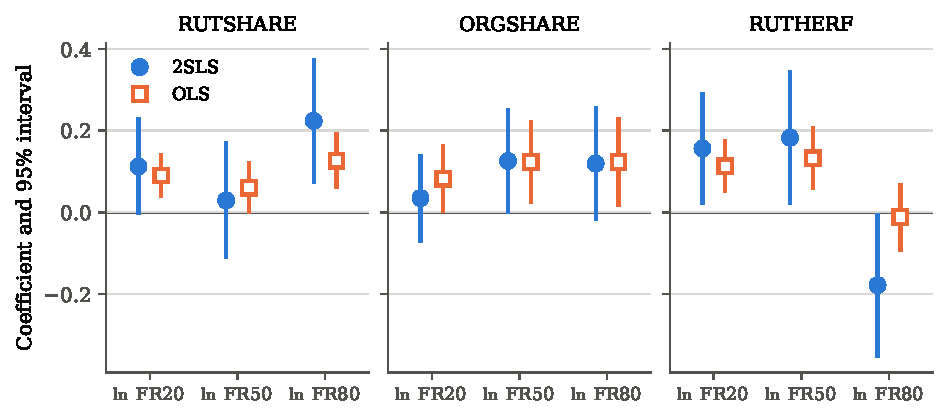
\includegraphics[width=0.97\linewidth]{figures/ch09/borenstein_coefs.pdf}
\caption{Market-power coefficients of the pricing equation by fare percentile, with 95\% confidence intervals
(estimate plus or minus 1.96 standard errors). Filled circles are 2SLS estimates and hollow squares OLS
estimates. The route-share and airport-share effects are positive at every percentile. The route-Herfindahl
effect, which holds the carrier's own share fixed, changes sign at the 80th percentile. Redrawn from
\citet{Borenstein1989}, Table 2.}
\label{fig:09-bor-coefs}
\end{figure}

Route share raises fares. Holding route concentration fixed, a one percentage point increase in a carrier's
route share raises its fares by between 0.03\% (FR50) and 0.22\% (FR80) (p.~357). Consider a dominant carrier
with 70\% of a route and rivals with 10\% each. All of them face the same route Herfindahl index, so the
comparison holds RUTHERF fixed automatically. The fare gap in log points is
\begin{equation*}
0.60 \times 0.1120 = 0.067, \qquad 0.60 \times 0.0288 = 0.017, \qquad 0.60 \times 0.2238 = 0.134
\end{equation*}
for FR20, FR50 and FR80. Borenstein summarizes this as a premium ``from 2\% to 12\%.''\footnote{The
arithmetic gives 1.7\% to 13.4\% in log points, or 1.7\% to 14.4\% as exact percentage changes
$e^{0.60\,\hat\phi_3} - 1$. The author's rounded range understates the upper end.} The effect is larger on the
20th and 80th percentiles than on the median, which Borenstein finds surprising. Yet a \emph{Chow test}, here a
test of whether a coefficient is equal across the three percentile regressions, does not reject equality
(p.~358). Only the FR80 coefficient is significant at 1\%. The FR20
coefficient is significant at 10\%, and the FR50 coefficient is not significant.

Airport share also raises fares, and more so at the high end of the fare distribution. The FR80 coefficient on
ORGSHARE, 0.1191, is about three times the FR20 coefficient, 0.0345, and Borenstein reports that the difference
is significant at 10\% (p.~358). Travelers who pay full coach fares are much more likely to be active members
of frequent-flyer programs than travelers on deep discounts. A stronger effect on high fares therefore fits the
FFP mechanism. A one standard deviation increase in ORGSHARE, 0.1305, raises the three log fares directly by
\begin{equation*}
0.1305 \times 0.0345 = 0.0045, \qquad 0.1305 \times 0.1254 = 0.0164, \qquad 0.1305 \times 0.1191 = 0.0155,
\end{equation*}
which the paper rounds to 0.5\%, 1.6\% and 1.6\%. Consider a carrier with half the originations at both
endpoints. It charges median and high-end fares about $0.5 \times 0.12 = 0.06$, or 6\%, above those of a
carrier with a very small presence at the two airports (p.~358).

These figures ignore an indirect channel. Airport dominance also raises a carrier's share of every route from
the airport. Borenstein estimates the size of this channel in a companion discussion paper, ``The Competitive
Advantage of a Dominant Airline'' (p.~358).\footnote{University of Michigan, Institute of Public Policy Studies,
Discussion Paper 280, 1989, as listed in the article's references. We cite it in the text only, so that its year
does not collide with the article's in the bibliography.} A one point increase in a carrier's share of originations at an airport raises its share of a route by up to 0.33
points, depending on its initial share. At the FR80 coefficient on route share, the indirect channel adds at most
$0.33 \times 0.2238 = 0.074$ to the direct ORGSHARE coefficient of 0.1191. When RUTSHARE and RUTHERF are dropped
from the equation, a one point increase in ORGSHARE raises the three percentiles by 0.24\%, 0.26\% and 0.24\%,
each significant at 1\% (p.~360, n.~46). These reduced-form effects exceed the sums of the direct and maximal
indirect effects implied by \cref{tab:09-bor-main}, which are 0.07, 0.13 and 0.19 per unit of
ORGSHARE.\footnote{The sums are $0.0345 + 0.33 \times 0.1120$, $0.1254 + 0.33 \times 0.0288$ and
$0.1191 + 0.33 \times 0.2238$. This comparison is our calculation.} By the omitted-variable formula, the
reduced-form coefficient picks up the full sample association of airport share with route share and route
concentration, which can exceed the causal channel.

Route concentration, holding the carrier's own share fixed, has mixed effects. It raises low-end and median fares
and lowers high-end fares, and all three coefficients are significant at 5\%. Borenstein illustrates with a
merger. Let firm 1 carry half of a route's passengers and two rivals a quarter each. A merger of the two rivals
changes the route Herfindahl index from
\begin{equation*}
0.5^2 + 2 \times 0.25^2 = 0.375 \qquad \text{to} \qquad 0.5^2 + 0.5^2 = 0.5,
\end{equation*}
an increase of 0.125, slightly more than half a standard deviation ($\frac{0.125}{0.2237} = 0.56$). Holding
firm 1's share fixed, its log fares change by
\begin{equation*}
0.125 \times 0.1559 = 0.019, \qquad 0.125 \times 0.1822 = 0.023, \qquad 0.125 \times (-0.1787) = -0.022
\end{equation*}
at the three percentiles. The paper reports the first and last, a 1.9\% rise in the low-end fare and a 2.2\%
fall in the high-end fare (p.~358). Endpoint concentration may lower low-end fares and raise high-end fares,
but none of the ORGHERF coefficients differs significantly from zero.

The cost and quality coefficients mostly have the expected signs when they are significant (pp.~358--359). The
elasticities of fares with respect to distance (0.33 to 0.41) and rivals' costs (0.50 to 0.84) are positive and
below one. Load factor has a negative coefficient, significant only for FR20, where a 10\% higher load factor
lowers the fare by about 0.75\%. Frequency has positive elasticities of 0.014, 0.024 and 0.043, larger for high
fares, and a Chow test rejects their equality across percentiles (p.~358, n.~41). Business travelers value
frequent service most.

Borenstein adds a caution about the frequency premium (p.~358, n.~42). In a competitive market, higher quality
would raise price only if it raised cost. After controlling for load factor, frequent flights may even be
cheaper, because they allow more intensive use of ground labor. The frequency premium may therefore reflect
market power more than a payment for quality.

Each on-plane stop lowers fares by 3\% to 13\% and each change of plane by 3\% to 8\%, so lower-quality products
sell for less. Circuity, holding stops and changes fixed, raises fares significantly but modestly. At the mean
circuity of 1.0754, the effect is $0.1458 \ln 1.0754 = 0.011$ at FR20 and $0.2062 \ln 1.0754 = 0.015$ at FR80,
which brackets the author's ``about 1.4\%'' (p.~359). A trip with one change of plane has a lower
80th-percentile fare than a nonstop trip if
\begin{equation*}
-0.0616 + 0.2062 \ln \mathit{CIRC} < 0
\qquad \Longleftrightarrow \qquad
\ln \mathit{CIRC} < \frac{0.0616}{0.2062} = 0.299 .
\end{equation*}
With the approximation $\ln \mathit{CIRC} \approx \mathit{CIRC} - 1$, the extra mileage may not exceed about 30\%
of the nonstop distance, the figure in the paper. The exact bound is $e^{0.299} - 1 = 0.35$, or 35\%.

Tourism lowers fares, with elasticities of $-0.019$, $-0.056$ and $-0.099$, so the effect grows toward the high
end of the distribution. Borenstein's reading is that on leisure routes carriers do not cut their deepest
discounts much. Instead they make more seats available at moderate discounts and at unrestricted discount fares
(p.~359).

\casehead{Carrier effects and scarcity rents} All carrier constants differ significantly from zero (p.~359). The
gap between the highest and the lowest carrier is 30\% for FR20 and 20\% for FR80. Holding all regressors
fixed, Continental, Eastern and Piedmont charge the lowest fares and United and Delta the highest. The scarcity
estimates are positive and significant at the two largest airports, O'Hare (3\% to 5\%) and Atlanta (1\% to
3\%), and at Denver (2\% to 4\%) and Cleveland (0\% to 3\%). Ten airports show consistently negative and
significant effects, mostly between 1\% and 7\% (p.~359, n.~43). They are Dallas/Fort Worth, Los Angeles,
Newark, La Guardia, Kennedy, Miami, Houston Intercontinental, Las Vegas, Kansas City and Fort Lauderdale. The
paper does not state the route distance at which these percentages apply. Under the scaling of
\cref{eq:09-bor-apt}, a coefficient $\varrho_k$ is the effect on a 1,000-mile route.

The negative estimates are puzzling for a measure of scarcity rents, which cannot be negative. They are
especially puzzling at La Guardia and Kennedy, which were slot-controlled. Three features of the design may
explain them. The airport terms absorb any airport-specific cost or demand factor, such as local fuel prices or
wages (p.~351, n.~26), in addition to rents. Several of the negative airports serve leisure destinations, such
as Las Vegas, Miami and Fort Lauderdale, whose travel mix the tourism index may capture imperfectly. Newark, La
Guardia and Kennedy also compete for New York travelers, while the model treats each airport as a separate
market. Dropping the distance scaling changes the results for some airports noticeably (p.~354, n.~34), so the
airport estimates are sensitive to functional form as well.

\casehead{Potential competition} Adding POTCOMP leaves the other estimates nearly unchanged (Panel B of
\cref{tab:09-bor-main}). The RUTSHARE coefficients rise slightly, to 0.1196, 0.0564 and 0.2470, and the FR80
coefficient on RUTHERF becomes more negative. POTCOMP itself has negative coefficients, significant at 5\% for
FR20 only. The effect is small. A one standard deviation increase in POTCOMP, 0.159, lowers the log fare by
$0.159 \times 0.0589 = 0.009$ at FR20 and by less at the other percentiles (p.~359). Any endogeneity bias in
POTCOMP points in the negative direction, so the true effect may be smaller still.

\casehead{Least squares} The OLS estimates in Panel B tell the same qualitative story with smaller standard
errors. The OLS route-share coefficients, 0.0899, 0.0596 and 0.1259, lie below the 2SLS estimates at FR20 and
FR80 and above them at FR50. By \cref{eq:09-bor-olsbias}, OLS understates the share effect when the simultaneity
term $b_s\sigma_u^2$ outweighs the quality term $\sigma_{uv}$, which fits the two tails. The OLS
route-Herfindahl coefficients are positive and significant for FR20 and FR50 and near zero for FR80.

\casehead{The relative-price equation} \Cref{tab:09-bor-rel} reproduces Table 3 of the paper. The first three
columns estimate \cref{eq:09-bor-rel}, and the last three drop the difference in route shares. In the full
equation, the route-share and airport-share coefficients have the signs found in \cref{tab:09-bor-main}, but
none is individually significant. Their standard errors are two to three times those in
\cref{tab:09-bor-main}.

\begin{table}[htbp]
\centering
\caption{The relative-price equation: estimates of \cref{eq:09-bor-rel}}
\label{tab:09-bor-rel}
\footnotesize
\begin{tabular}{@{}lcccccc@{}}
\toprule
& \multicolumn{3}{c}{Equation (4)} & \multicolumn{3}{c}{RUTSHARE excluded} \\
\cmidrule(lr){2-4} \cmidrule(l){5-7}
Dependent variable & $\ln$ FR20 & $\ln$ FR50 & $\ln$ FR80 & $\ln$ FR20 & $\ln$ FR50 & $\ln$ FR80 \\
\midrule
$\ln$ LOADFAC & 0.0277 & 0.0713$^{\dagger}$ & 0.0727$^{\dagger}$ & 0.0307 & 0.0790$^{*}$ & 0.0793$^{*}$ \\
 & (0.0254) & (0.0348) & (0.0350) & (0.0246) & (0.0325) & (0.0329) \\
$\ln$ EQUIP & $-0.0239$ & $-0.0293$ & $-0.0161$ & $-0.0148$ & $-0.0065$ & 0.0036 \\
 & (0.0224) & (0.0307) & (0.0309) & (0.0168) & (0.0222) & (0.0225) \\
$\ln$ FREQ & 0.0116 & 0.0038 & 0.0115 & 0.0183$^{*}$ & 0.0209$^{\dagger}$ & 0.0263$^{*}$ \\
 & (0.0131) & (0.0179) & (0.0180) & (0.0071) & (0.0094) & (0.0095) \\
$\ln$ CIRC & 0.0955 & 0.2309$^{\dagger}$ & $-0.0793$ & 0.0509 & 0.1181$^{\dagger}$ & $-0.1768^{*}$ \\
 & (0.0845) & (0.1156) & (0.1163) & (0.0434) & (0.0574) & (0.0581) \\
STOP & $-0.0688^{*}$ & $-0.0983^{*}$ & $-0.0589$ & $-0.0599^{*}$ & $-0.0759^{\dagger}$ & $-0.0396$ \\
 & (0.0290) & (0.0396) & (0.0399) & (0.0248) & (0.0328) & (0.0332) \\
PLANECHG & $-0.0690$ & $-0.0722$ & $-0.0765$ & $-0.0946^{*}$ & $-0.1370^{*}$ & $-0.1325^{*}$ \\
 & (0.0437) & (0.0598) & (0.0601) & (0.0137) & (0.0181) & (0.0183) \\
ORGSHARE & 0.0013 & 0.0275 & 0.1393 & 0.0742$^{\dagger}$ & 0.2117$^{*}$ & 0.2986$^{*}$ \\
 & (0.1234) & (0.1688) & (0.1698) & (0.0360) & (0.0476) & (0.0482) \\
RUTSHARE & 0.0929 & 0.2346 & 0.2029 & & & \\
 & (0.1501) & (0.2053) & (0.2065) & & & \\
\addlinespace
$R^2$ & 0.269 & 0.193 & 0.196 & 0.310 & 0.268 & 0.262 \\
Observations & 1,508 & 1,508 & 1,508 & 1,508 & 1,508 & 1,508 \\
\bottomrule
\end{tabular}

\smallskip
\begin{minipage}{0.95\linewidth}
\footnotesize Notes: Each variable enters as the difference between the two carriers on a route. Standard
errors in parentheses, asymptotic for equation (4). Significance marks as printed in the paper: $^{\#}$ 10\%,
$^{\dagger}$ 5\%, $^{*}$ 1\%. Carrier effects are included but not reported. Source: \citet{Borenstein1989},
Table 3.
\end{minipage}
\end{table}

Borenstein traces the imprecision to two sources (p.~359). First, the instrument for the difference in route
shares is less effective than GENPSH is in the pricing equation, though still significant. The fitted share
difference is therefore closer to a linear combination of the other regressors. Second, the differences in
RUTSHARE and ORGSHARE between two carriers on the same route are much more highly correlated than the levels in
the pricing equation. A test of the joint significance of the two share differences rejects zero at 1\% for all
three fare percentiles.\footnote{Several coefficients that the paper marks as significant at 1\% have $t$
statistics between 2.33 and 2.58. Examples are $\ln$ FREQ in the 2SLS FR50 column of Table 2 ($t = 2.51$) and STOP
in the FR20 column of Table 3 ($t = 2.37$). These marks match one-sided rather than two-sided cutoffs. We
reproduce the marks as printed.}

Dropping the route-share difference confirms the diagnosis of collinearity. The ORGSHARE coefficients rise to
0.0742, 0.2117 and 0.2986, and their standard errors fall to under a third of their previous size. Dropping the
ORGSHARE difference instead raises the RUTSHARE coefficients and lowers their standard errors (p.~360, n.~45).
Without the route-share term, the ORGSHARE coefficients measure the direct effect of airport share plus its
indirect effect through route share. A carrier with 50\%
of the traffic at each endpoint charges high-end fares $0.40 \times 0.2986 = 0.119$ log points, about 12\%,
above a rival with 10\% at each endpoint (p.~360). The corresponding gaps at FR20 and FR50 are 0.030 and 0.085
log points.

The other coefficients agree with those of the pricing equation when significant, with one exception. Load
factor now has positive coefficients, significant for FR50 and FR80. Across routes, denser routes with higher
load factors may have lower fares. Within a route, the carrier with the higher load factor may carry more
connecting traffic, which raises the opportunity cost of its seats and hence its fares (p.~360).

\casehead{Robustness} The paper reports several further checks, mostly in footnotes.
\begin{itemize}
\item Airport shares based on enplanements instead of originations change the results very little (p.~349).
\item Treating Continental and Eastern as one firm in the share calculations changes the results slightly. The
changes reinforce the finding that large airport and route shares yield market power (p.~349, n.~20).
\item The signs and approximate significance are robust to logs instead of levels of the shares and Herfindahl
indices in \cref{eq:09-bor-price} (p.~354), and of the shares in \cref{eq:09-bor-rel} (p.~355).
\item The aircraft-size coefficient does not differ between routes with average flight lengths above and below
500 miles, and the two estimates are very similar (p.~350, n.~22).
\item Scarcity variables without the distance scaling yield similar route-share and airport-share effects,
though some airport estimates change noticeably (p.~354, n.~34).
\item In \cref{eq:09-bor-rel}, a proportional fare difference that varied with distance would make the errors
heteroskedastic. Regressions of the squared residuals on DISTANCE give $t$ statistics below one for all three
percentiles (p.~355, n.~36).
\item Treating LOADFAC as endogenous leaves the market-power conclusions intact (p.~357, n.~38).
\end{itemize}

\subsection{From descriptive results to economic inferences}\label{sec:09-bor-inference}

Regression coefficients describe conditional correlations. They become economic conclusions only through a
chain of reasoning that rules out alternatives. We reconstruct Borenstein's chain one conclusion at a time,
with the evidence and the test behind each step. \Cref{tab:09-bor-hyp} lists the competing hypotheses, their
predictions for the two equations, and the verdict of the evidence.

\begin{table}[htbp]
\centering
\caption{Hypotheses, predictions and evidence in Borenstein (1989)}
\label{tab:09-bor-hyp}
\footnotesize
\renewcommand{\arraystretch}{1.15}
\begin{tabularx}{\linewidth}{@{}>{\raggedright\arraybackslash}p{0.2\linewidth}
  >{\raggedright\arraybackslash}X >{\raggedright\arraybackslash}X@{}}
\toprule
Hypothesis & Prediction & Evidence \\
\midrule
Perfect contestability & $\phi_1 = \phi_2 = \phi_3 = \phi_4 = 0$ in \cref{eq:09-bor-price}. & Rejected. RUTSHARE
and ORGSHARE raise fares (\cref{tab:09-bor-main}). The share differences are jointly significant at 1\%
(\cref{tab:09-bor-rel}). \\
Collusive umbrella & $\phi_4 > 0$ at every percentile. Under a complete umbrella, $\phi_3 = 0$ in
\cref{eq:09-bor-rel}. & Not supported. $\phi_4 > 0$ for FR20 and FR50 but $\phi_4 < 0$ for FR80. The carrier
with the larger shares charges more than its rival on the same route. \\
Carrier-specific dominance (\cref{prop:09-dominance}) & $\phi_1, \phi_3 > 0$ in both equations. $\phi_4$ may be
negative. & Supported by the own-share effects in both equations and by the absence of a consistent umbrella. \\
Frequent-flyer mechanism & ORGSHARE effect larger for high fares than for low fares. & Supported. The FR80
coefficient is about three times the FR20 coefficient, and the difference is significant at 10\%. \\
Scarcity rents & $\varrho_k > 0$ and equal for all carriers at airport $k$. & Mixed. Positive at O'Hare,
Atlanta, Denver and Cleveland, negative at ten airports. \\
Quality premia & Positive frequency effect, larger for high fares. & Found, but the premium may reflect market
power (p.~358, n.~42). \\
\bottomrule
\end{tabularx}

\smallskip
\begin{minipage}{\linewidth}
\footnotesize Notes: The hypotheses are stated in terms of the coefficients of \cref{eq:09-bor-price} and
\cref{eq:09-bor-rel}. The first row corresponds to prediction (C1) of \cref{sec:09-contest-fail}.
\end{minipage}
\end{table}

The first conclusion is that dominance raises a carrier's own fares. The evidence is the positive RUTSHARE and
ORGSHARE coefficients in \cref{tab:09-bor-main}. The Hausman test shows that route share is endogenous, and the
estimates that support the conclusion instrument it with GENPSH. The relative-price equation then removes every
route-level unobservable. The joint test of the share differences in \cref{tab:09-bor-rel} still rejects zero
at 1\%.

The second conclusion is that the dominant carrier's market power does not spill over to its rivals. Two
results support it. Holding the carrier's own share fixed, route concentration raises low-end fares but lowers
high-end fares. An umbrella would raise all of them. Within a route, the carrier with the larger shares charges
more, while a complete umbrella would equalize fares. In the paper's words, ``the market power of a dominant
airline does not spill over substantially to other airlines serving the same airport or routes'' (p.~362).

The third conclusion concerns mechanisms. The airport-share effect is concentrated in high fares, which are paid
mostly by business travelers who belong to frequent-flyer programs. This pattern fits FFPs and TACOs. The
evidence cannot separate the individual devices, however, or rule out other sunk costs of entry, such as
advertising and the setup of airport facilities (p.~362). The fourth conclusion is that scarcity rents are a separate
phenomenon. Because the airport terms are common to all carriers at an airport, they cannot absorb the
carrier-specific effect of airport share.

Borenstein considers several alternative explanations. Scarcity rents are handled by the airport terms. Quality
differences are handled by the service variables, with the caution that their coefficients need not be quality
premia. The cash value of frequent-flyer bonuses could explain the airport-share effect only in part. Realistic
calculations put that value at one or two percentage points of fares at most \citep{Borenstein1988}, and deeply
discounted travelers rarely redeem mileage (p.~358, n.~39). The loyalty-inducing effect of the bonuses can still
be large if their kickback aspect matters. Potential competition is handled by POTCOMP and the endogeneity of
load factor by the Hausman test.

The asymmetry between a dominant carrier's fares and its rivals' fares maps directly into the theory of
\cref{sec:09-pricing}. In the conduct model with collusiveness rising in concentration, every carrier's markup
rises with the route Herfindahl index, so concentration lifts the fares of small carriers too. In the
differentiated-products model of \cref{prop:09-dominance}, an increase in one carrier's attractiveness, from
FFP value or reputation, raises its price and share and lowers its rivals' prices. By \cref{cor:09-relprice},
the dominant carrier's price relative to its rivals' then rises with the share gap, which is the pattern of
\cref{tab:09-bor-rel}. Borenstein's evidence fits the second model.

The policy conclusion is measured. ``It would be futile and probably unwise for the government to try to deter
airlines from forming hubs'' (p.~360). Borenstein cites substantial evidence that hub-and-spoke systems use
aircraft and other inputs more efficiently than the point-to-point systems of the regulated era. Hub operations
may bring cost savings that raise total surplus even if carriers keep them as profit. They may also bring more
frequent flights, easier connections and more nonstop service. These benefits must be weighed against the higher
fares that airport dominance brings (p.~362). \citet{CarltonLandesPosner1980} propose one way to analyze such
benefits (p.~362, n.~47).

The quality coefficients should not be read as hedonic prices for this welfare calculation (p.~362, n.~48).
Quality also affects cost, which confounds the coefficients. Even without that problem, \citet{Spence1975}
showed that a firm with market power chooses quality to suit the marginal consumer. If inframarginal travelers
value quality more than marginal ones, as is likely in air travel, the coefficients reflect the marginal
traveler's valuation. They then underestimate the average traveler's valuation of hub service.

\subsection{Limitations and critiques}\label{sec:09-bor-critiques}

The first critique is the one \citet{Demsetz1973} raised against structure-conduct-performance regressions
(\cref{ch:intro}). A large route or airport share may reflect a better product or a lower cost instead of
market power. \citet[pp.~5--6]{BerryCarnallSpiller2006} press this point. Reduced-form price regressions do not
show how prices relate to costs or what determines markups over cost. Ticket restrictions, which explain much
of the variation of fares within a route, are absent from the data, and earlier studies could not control for
them. Their response is to model demand, with an explicit unobserved product characteristic, together with
costs and equilibrium pricing (\cref{sec:09-bcs}).

A related limitation is that the paper has no explicit cost function. Following \citet{Bresnahan1989},
Borenstein infers costs from cross-sectional variation in prices and product attributes (p.~348, n.~18). The
coefficients of the cost and quality variables therefore mix cost and demand effects. Markups and marginal costs
are not separately identified, which is the gap that a structural model fills.

\citet[p.~446]{WhinstonCollins1992} raise two critiques that apply to all pricing regressions of the period.
These studies treat their samples as sets of unrelated routes, although the routes form an interrelated network.
The effective cost of serving a route depends on where the plane can fly next (p.~446, n.~2). The studies
also need controls for demand and cost conditions, and market-structure variables are likely to be correlated
with what the controls miss. Their event study is designed to avoid both problems (\cref{sec:09-wc}).

The exclusion restriction for GENPSH is open to doubt, as Borenstein acknowledges. Later evidence sharpens the
doubt. \citet{GoolsbeeSyverson2008} identify routes on which Southwest becomes a credible entrant because it
begins operating at the second endpoint. Incumbents cut fares significantly in response, before Southwest starts
flying the route. In the working-paper version of their study, operating at both endpoints goes with a
probability of entering the route about 70 times higher than on other routes. This finding supports the
relevance of a both-endpoints instrument and contradicts its exclusion. By \cref{eq:09-bor-ivbias}, fare cuts
against potential entrants bias the 2SLS share effect upward, so the route-share coefficients in
\cref{tab:09-bor-main} may overstate the effect of route dominance.

Several regressors that the paper treats as exogenous are equilibrium outcomes. Borenstein acknowledges this for
the service variables. The same concern applies to ORGSHARE, since a carrier's fares affect how many travelers
begin their trips with it at an airport. The paper instruments route share but not airport share. If high
unobserved quality raises both airport share and fares, the ORGSHARE coefficients overstate the effect of
dominance.

The pricing equation imposes a common share coefficient on routes with different elasticities and conduct. By
\cref{eq:09-pricing-approx}, $\phi_3$ then estimates an average of $\frac{1 - \eta_t}{\varepsilon_t}$ across
routes, weighted by the identifying variation, and the same holds for $\phi_4$. The conduct-parameter literature
raises the same concern about reading an estimated conduct parameter as a structural constant
(\citealp{Corts1999}, \cref{ch:conduct}). Even a precise $\phi_3$ cannot separate elastic demand from nearly
collusive conduct without outside information on $\varepsilon$ (\cref{rem:09-share-coef}).

The design uses a single cross-section and one carrier per route. Without time variation, only the
relative-price equation controls for unobserved route characteristics, and that equation is imprecise because of
collinearity and a weaker instrument. Fare percentiles mix fare classes whose restrictions are unobserved, so a
high FR80 may reflect a carrier's mix of restricted and unrestricted tickets as well as its markup. Finally,
airports in the same city are treated as separate markets. \Cref{sec:09-wc} studies entry by a low-fare carrier
on routes from Newark. The entry reduced the value of incumbents on the entered airport pairs much more than the
value of carriers serving the same city pairs from other New York airports. That evidence supports treating airports in a
city as differentiated products, a weaker assumption than treating them as separate markets.

\subsection{Contribution}\label{sec:09-bor-contribution}

The paper made four contributions. First, it provided the first systematic evidence that a carrier's dominance
of its endpoint airports predicts its fares, beyond the concentration of the route. This moved the policy debate
from route concentration to airport concentration. Second, it documented an asymmetry. Dominant carriers charge
more, and their rivals do not share in the premium. The finding shifted the interpretation of the
concentration-price correlation from collusion toward carrier-specific advantages, such as those created by
FFPs, TACOs and reservation systems.

Third, the paper introduced two identification devices that later work adopted. Scarcity rents are separated
from market power by restricting airport effects to be common across carriers, and presence at both endpoints of
a route serves as a shifter of route share. Fourth, by estimating separate equations for three fare
percentiles, the paper showed that market power and quality premia differ across fare types. This heterogeneity
anticipated the two-type demand model of \citet{BerryCarnallSpiller2006}.

The paper also set the agenda for the other two studies of this chapter. \citet{WhinstonCollins1992} measure
route-specific rents without the cost and demand controls that a pricing regression needs.
\citet{BerryCarnallSpiller2006} separate markups from costs and explain the absence of an umbrella through the
sorting of business travelers. \citet{Borenstein1991} pursued the question with directional city-pair effects
\citep[p.~5]{BerryCarnallSpiller2006}. Comparing routes into and out of a hub city, he found higher fares on
flights out of the hub.

\begin{table}[htbp]
\centering
\caption{Identification and counterfactual map of Borenstein (1989)}
\label{tab:09-bor-map}
\footnotesize
\renewcommand{\arraystretch}{1.1}
\begin{tabularx}{\textwidth}{@{}>{\raggedright\arraybackslash}p{2.6cm}>{\raggedright\arraybackslash}X@{}}
\toprule
Observed data & The DOT ticket sample for the third quarter of 1987, with service segment and nonstop market
  data. Fare percentiles, route and endpoint shares and Herfindahls, and cost and quality variables for one
  carrier on each of 3,591 airport-pair routes. \\
\addlinespace
Latent objects & Carrier-route markups and marginal costs, unobserved service quality, and route-level
  demand and cost shocks. \\
\addlinespace
Estimated parameters & The coefficients of \eqref{eq:09-bor-price} on market structure ($\phi_1$ to
  $\phi_6$) and on cost and quality ($\gamma_1$ to $\gamma_6$), carrier effects and 24 airport effects, for
  three fare percentiles. \\
\addlinespace
Identifying variation & Cross-route differences in dominance, with route share instrumented by GENPSH
  \eqref{eq:09-genpsh}, the carrier's share of geometric-mean endpoint enplanements. A relative-price
  equation differences out route-level unobservables. \\
\addlinespace
Maintained assumptions & GENPSH is excluded from the pricing equation. Shares do not proxy for unobserved
  quality or cost, airport share is exogenous, and the share coefficients are common across routes. \\
\addlinespace
Counterfactual and what it holds fixed & No equilibrium is simulated. The coefficients compare fares at
  different levels of dominance, holding the measured cost and quality variables fixed. \\
\addlinespace
Conclusion & A carrier with 70 percent of a route charges 2 to 12 percent more than rivals with 10 percent,
  and endpoint dominance raises high fares most. Rivals share little of the premium. The reading rests on
  the exclusion of the instruments. \\
\addlinespace
One limitation & Without a model of cost or demand, a high fare that reflects market power cannot be told
  apart from a high fare for a better product. \\
\addlinespace
Source and our additions & The four tables are Borenstein's. The bias formulas \eqref{eq:09-bor-olsbias}
  and \eqref{eq:09-bor-ivbias}, \cref{prop:09-dominance} and \cref{tab:09-bor-hyp} are our
  reconstructions. \\
\addlinespace
Tools in the appendices & \Cref{sec:A-iv,sec:A-ols}. \\
\bottomrule
\end{tabularx}
\end{table}
